\documentclass[a4paper]{article}

\usepackage[utf8]{inputenc}
\usepackage[T1]{fontenc}
\usepackage{textcomp}
\usepackage[english]{babel}
\usepackage{amsmath, amssymb}
\usepackage{natbib}
\usepackage{float} 
\usepackage[caption = false]{subfig}
\usepackage{listings}
\lstset{
    breaklines=true,
    basicstyle=\tt\normalsize,
    keywordstyle=\color{blue},
    identifierstyle=\color{magenta},
    frame = single
} 
% figure support
\usepackage{import}
\usepackage{xifthen}
\pdfminorversion=7
\usepackage{pdfpages}
\usepackage{transparent}
\pdfsuppresswarningpagegroup=1

\title{Assignment 3 \\ Segmentation}
\author{Linus Falk}
\begin{document}
\maketitle

\section{Introduction}
In this assignment we are asked to count the number of coins in a provided image. 

\section{Method}
Below is a Matlab script that solves the problem of counting coins (and classifiying them) presented. Each method is commented why its needed in the script.

\begin{lstlisting}[language=MATLAB]
I=imread('lab3_material/coins.tif');
subplot(2,3,1)
imshow(I) %Display input image

f=[1 1 1 1; 1 1 1 1; 1 1 1 1; 1 1 1 1;]./16; %filter away small sharp edges on coin surface
I=imfilter(I,f,'symmetric');
I = medfilt2(I); %Filer away bright pixels.
T = graythresh(I); % Find treshold to mask away background
I_2 = im2bw(I,T);   % create binary image of background and coins

%figure(1)
subplot(2,3,2)
imshow(I_2) %Display binary image


%figure(3)
subplot(2,3,3) 
Idist = bwdist(I_2,"euclidean"); %Calculate distance to edges
Idist = -Idist; %invert it for the next step
se = strel('disk',5); % try to remove small not connected parts of coins
Idist = imerode(Idist,se);
imshow(Idist,[]);


%figure(5)
subplot(2,3,4)
L = watershed(Idist); %watershed to isolate each coin after eroding
L(I_2) = 0; %set background to zero
rgb = label2rgb(L,'spring',[1 1 1]);
imshow(rgb)

%figure(6)
subplot(2,3,5)
T = 0;
I_2 = im2bw(L,T); % create a new binary image with all coins separated
imshow(I_2)

%figure(7)
subplot(2,3,6)
Ilabel=bwlabel(I_2,4); % label all objects, coins


stats = regionprops('table',I_2,'Centroid','MajorAxisLength','MinorAxisLength'); %get properties, center and majoraxis length
centers = stats.Centroid;
diameters = stats.MajorAxisLength;
radii = diameters/2;
imshow(I_2)
hold on
viscircles(centers,radii); %display all objects radii with circles, centered with majoraxis length
title('Radii','Interpreter','latex', 'fontsize',22)
hold off

figure(9)
radii(radii < 17) = []; % remove to small objects befor making histogram
hist(radii, 30)

figure(8)
F=regionprops(Ilabel,'Area');
A=[F.Area];
A(A<200) = []; 
hist(A)
title('Area','Interpreter','latex', 'fontsize',22)
\end{lstlisting}


\section{Result}
\begin{figure}[ht!]
\centering
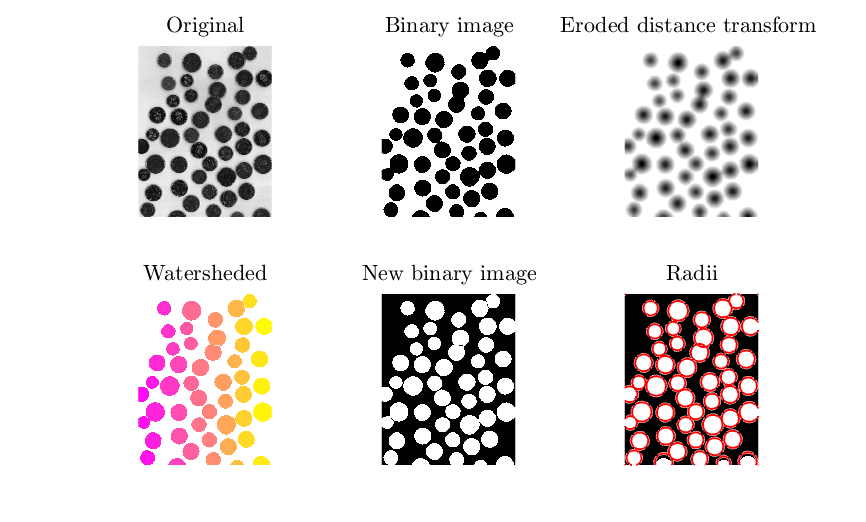
\includegraphics[width=130mm]{assign_3.png}
\caption{Example of caption}
\label{fig:example}
\end{figure}

\section{Result}
\begin{figure}[ht!]
\centering
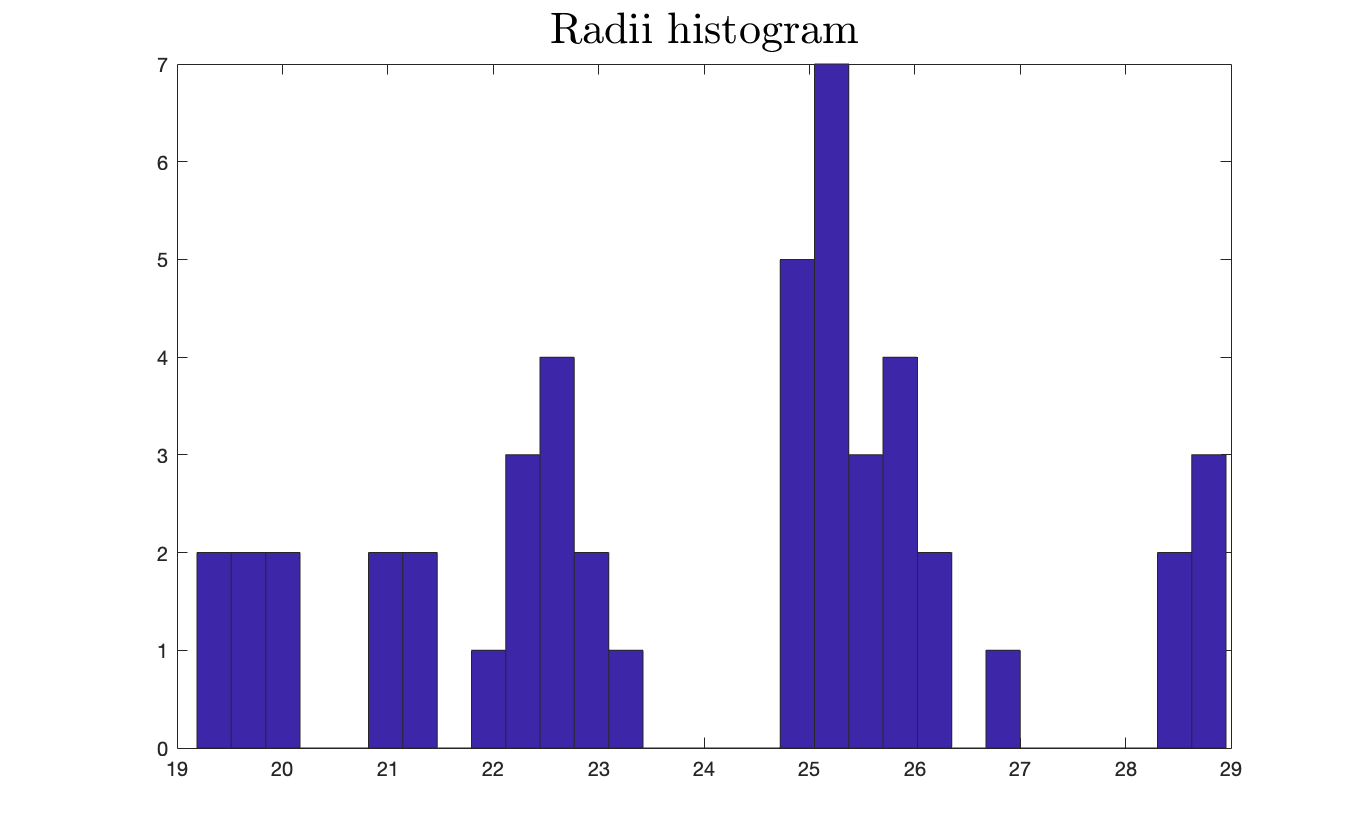
\includegraphics[width=130mm]{assign_3b.png}
\caption{Example of caption}
\label{fig:example2}
\end{figure}


\section{Discussion}

\textbf{A discussion of errors and limitations in your final method.}

The method can count all coins in the image but have problem with classifiying one of the coins. Better pre processing to avoid shadows being included as edge of the coin could be one solution. 

\textbf{As you can see, the objects are coins. Is it possible to count the total amount
of money using your algorithm?}
It is possible to count the sum of the money. More compex allgorithm would be needed if less then half of the coin is present in the image to correctly classify it with radius. In this model the objects longest axis is used to calculate the radii, by doing this we can approximate the radius and get a good classification of the partial image of the coins. 


\textbf{Explain how your method treat the coins on the image border.}
As described above is the majoraxis lenght used to identify the radii of the coins which works well as long as at least halft the coin is in the image. 



\textbf{Is your solution general in the sense that it can be used when analyzing im-
ages with arbitrary circular objects (i.e. not only coins.tif)?}


\bibliographystyle{unsrt}
\bibliography{references}
\end{document}